\documentclass[journal]{IEEEtran} 
\IEEEoverridecommandlockouts
% The preceding line is only needed to identify funding in the first footnote. If that is unneeded, please comment it out.
\usepackage{multirow}%,bigdelim}
\usepackage[hidelinks,draft]{hyperref} % draft is added to bypass issues seen with glossary terms broken up by line-breaks
\newcommand{\emaillink}[1]{\href{mailto:#1}{#1}}
\usepackage{url}
\usepackage{soul}
\usepackage{cite}
\usepackage{amsmath,amssymb,amsfonts}
\usepackage{bm}
\usepackage{mathtools}
\usepackage{siunitx}
\usepackage{xfrac}
% \usepackage{algorithmic}
\usepackage{graphicx}
\graphicspath{{figs/}}
\usepackage{tcolorbox}
\usepackage{textcomp}
\usepackage{xcolor}
\usepackage{siunitx}
\usepackage{xspace}
\usepackage[utf8]{inputenc}

% \usepackage{tablefootnote}
\usepackage[export]{adjustbox}

% tables
\usepackage{array}
\usepackage{booktabs}
\usepackage{multirow}
\usepackage{makecell}

% Spacing
\usepackage[final]{microtype} % font expansion + protrusion

% \setlist[description]{leftmargin=\parindent,labelindent=\parindent}
\def\BibTeX{{\rm B\kern-.05em{\sc i\kern-.025em b}\kern-.08em
    T\kern-.1667em\lower.7ex\hbox{E}\kern-.125emX}}
\usepackage[textsize=tiny]{todonotes}
% \usepackage[textsize=tiny,disable]{todonotes}
% Maximize margin width to still barely see the sides of todonotes
\setlength{\marginparwidth}{1.3cm}

% Define a todolist for checkboxes
\makeatletter
\let\labelindent\relax
\makeatother
\usepackage[inline]{enumitem}
\newlist{todolist}{itemize}{2}
\setlist[todolist]{label=$\square$}
\usepackage{pifont}
\newcommand{\cmark}{\ding{51}}%
\newcommand{\xmark}{\ding{55}}%
\newcommand{\done}{\rlap{$\square$}{\raisebox{2pt}{\large\hspace{1pt}\cmark}}%
\hspace{-2.5pt}}
\newcommand{\wontfix}{\rlap{$\square$}{\large\hspace{1pt}\xmark}}

% \ifCLASSOPTIONcompsoc
%   \usepackage[caption=false,font=normalsize,labelfont=sf,textfont=sf]{subfig}
% \else
%   \usepackage[caption=false,font=footnotesize]{subfig}
% \fi
\usepackage[caption=false,font=footnotesize]{subfig}
\usepackage{titlecaps}
\usepackage{algorithm,algpseudocode}

%%%%%%%%%%%%%%%%%%%%%%%%%%%%%%%%%%%%%%%%%%%%%%%%%%
% Common macros
%%%%%%%%%%%%%%%%%%%%%%%%%%%%%%%%%%%%%%%%%%%%%%%%%%

\newcommand{\hsia}{H-Si(100)-2$\times$1\@\xspace}
\newcommand{\hsib}{H-Si(111)-1$\times$1\@\xspace}

% referencing labels
\newcommand{\fref}[1]{\figurename~\ref{#1}}
\newcommand{\tref}[1]{\tablename~\ref{#1}}
\newcommand{\secref}[1]{Section~\ref{#1}}
\newcommand{\eref}[1]{Eq.~\eqref{#1}} %\eqref provided by amsmath
\newcommand{\appenref}[1]{Appendix~\ref{#1}}

% in-text functions
\newcommand{\tsps}[1]{\textsuperscript{#1}}  % text superscripts
\newcommand{\tsbs}[1]{\textsubscript{#1}}  % text superscripts
\newcommand{\sref}[1]{\protect\subref{#1}}  % subfig referencing in main caption
\newcommand{\bpar}[1]{(\textbf{#1})}        % bolt text in parentheses

% To-do items
\newcommand{\TODO}[1]{\textcolor{red}{TODO: #1}}
\newcommand{\TODOlow}[1]{\textcolor{blue}{TODO: #1}}
\newcommand{\PLAN}[1]{
    \begin{tcolorbox}[colback=blue!30!white, % Background color
                      colframe=blue!60!black, % Frame color
                      boxsep=1pt, % Box padding
                      arc=2pt, % Corner rounding
                      boxrule=1pt] % Frame thickness
        \tiny
        #1
    \end{tcolorbox}
}
\newcommand{\OLD}[1]{\textcolor{lightgray}{#1}}

% math operators
\DeclareMathOperator\erf{erf}
\DeclarePairedDelimiter\ceil{\lceil}{\rceil}
\DeclarePairedDelimiter\floor{\lfloor}{\rfloor}
\newcommand{\vect}[1]{\boldsymbol{\mathbf{#1}}}
\DeclareSIUnit\angstrom{\text {Å}}

% Terms/math
\newcommand{\etal}{\textit{et al.}}

% \renewcommand{\baselinestretch}{0.99}

% Make \gls output with first letter of each word capitalized, not just first word
\usepackage{mfirstuc}

\makeatletter
\let\oldmakefirstuc\makefirstuc
\renewcommand*{\makefirstuc}[1]{%
  \def\gls@add@space{}%
  \mfu@capitalisewords#1 \@nil\mfu@endcap
}
\def\mfu@capitalisewords#1 #2\mfu@endcap{%
  \def\mfu@cap@first{#1}%
  \def\mfu@cap@second{#2}%
  \gls@add@space
  \oldmakefirstuc{#1}%
  \def\gls@add@space{ }%
  \ifx\mfu@cap@second\@nnil
    \let\next@mfu@cap\mfu@noop
  \else
    \let\next@mfu@cap\mfu@capitalisewords
  \fi
  \next@mfu@cap#2\mfu@endcap
}
\makeatother

\usepackage[acronym]{glossaries}

% Disable hyperlinks for glossary entries
\glsdisablehyper

% ML
\newacronym{ai}{AI}{artificial intelligence}
\newacronym{ml}{ML}{machine learning}
\newacronym{llm}{LLM}{large language model}
\newacronym{qat}{QAT}{quantization-aware training}
\newacronym{api}{API}{application programming interface}

% ML Accel
\newacronym{mvm}{MVM}{matrix--vector multiplication}
\newacronym{mxu}{MXU}{matrix multiply unit}
\newacronym{mac}{MAC}{multiply--accumulate}

% Atomic/Nanotech/Physics
\newacronym{stm}{STM}{scanning tunneling microscope}
\newacronym{afm}{AFM}{atomic force microscope}
\newacronym{set}{SET}{single-electron transistor}
\newacronym{bdl}{BDL}{binary-dot logic}

% Field-Coupled Nanocomputing
\newacronym{fcn}{FCN}{field-coupled nanocomputing}
\newacronym{sidb}{SiDB}{silicon dangling bond}
\newacronym{qca}{QCA}{quantum-dot cellular automata}
\newacronym{nml}{NML}{nanomagnetic logic}

% Devices
\newacronym{hal}{HAL}{hardware abstraction layer}
\newacronym{pi}{PI}{primary-input}
\newacronym{io}{I/O}{input/output}
\newacronym{adc}{ADC}{analog-to-digital converter}
\newacronym{cmos}{CMOS}{complementary metal-oxide-semiconductor}
\newacronym{cad}{CAD}{computer-aided design}
\newacronym{tpu}{TPU}{tensor processing unit}
\newacronym{alu}{ALU}{arithmetic logic unit}

% Architecture
\newacronym{pe}{PE}{processing element}

% EDA
\newacronym{rtl}{RTL}{register-transfer level}
\newacronym{eda}{EDA}{electronic design automation}
\newacronym{aig}{AIG}{and-inverter graph}

% fiction-specific algorithms
\newacronym{gold}{\emph{gold}}{graph-oriented layout design}
\newacronym{plo}{\emph{PLO}}{post-layout optimization}

% Others
\newacronym[longplural={figures of merit}]{fom}{FoM}{figure of merit}

\newcommand{\applyalwaysshortacros}{%
  \glsunset{ai}%
  \glsunset{ml}%
  \glsunset{llm}%
  \glsunset{cmos}%
  \glsunset{cad}%
}

\applyalwaysshortacros

% solve error: Page 1 has margin impositions
\def\IEEEtitletopspace{18pt}

\clubpenalty = 10000
\widowpenalty = 10000
\displaywidowpenalty = 10000

\begin{document}

\title{RTL-to-Atoms Synthesis of a Machine Learning Accelerator on Atomic-Scale Computers}

% \author{Anonymous author(s)}
\author{%
    Samuel~S.~H.~Ng, %
    Marcel Walter, %
    Simon Hofmann, %
    Jan Drewniok, %
    Robert Wille, %
    and Konrad Walus%
    % \thanks{This work was supported by the Natural Sciences and Engineering Research Council of Canada under Grant \mbox{RGPIN-2022-04830}.}%
    \thanks{S.~S.~H.~Ng and K.~Walus were with the Department of Electrical and Computer Engineering, University of British Columbia, Vancouver, BC, Canada (\mbox{\{samueln, konradw\}@ece.ubc.ca}); M.~Walter, S.~Hofmann, J.~Drewniok, and R.~Wille were with the Chair for Design Automation, Technical University of Munich, BY, Germany (\mbox{\{marcel.walter, simon.t.hofmann, jan.drewniok, robert.wille\}@tum.de}). M.~Walter, S.~Hofmann, and R.~Wille were also with the Munich Quantum Software Company GmbH, Garching near Munich, BY, Germany. R.~Wille was also with the Software Competence Center Hagenberg (SCCH) GmbH, Hagenberg, O\"O, Austria.}%
}

% \section*{Extension Plan}

% \subsection*{Main objectives}

% Objectives that, together, satisfy \SI{50}{\percent} new contents rule:
% %
% \begin{todolist}
%     \item[\done] Implement ripple-carry adder and array multiplier in Verilog with a wrapper that automatically generates N-bit versions
%     \item[\done] Testbench the above for verification
%     \item[\done] In the Processing Element, replace multiplication and accumulation operations with the optimized \glspl{alu} \textcolor{orange}{using Yosys's technology mapper}
%     \item[\done] Synthesize and report changes
%     \item \textcolor{orange}{Post-Yosys equivalence check (use PE-forward test bench)}
%     \item[\done] \textcolor{orange}{Extend Verilogs to accept arbitrary width and activation bit-width settings}
%     \item New table similar to DATE's table: report multiple algorithm combinations (e.g., ortho with and without PLO, FoM vs. uniform gates), \textcolor{orange}{test multiple bit-widths (W8A8, W4A4, W2A2)}, report FoM-informed results similarly
%     \begin{itemize}
%         \item Further study possible with gold with different cost metrics (e.g., area vs crossing vs area-crossing product etc.)
%         \item Using CP as cost function might give us more squarish outputs
%     \end{itemize}
% \end{todolist}

% \subsection*{Stretch goals}

% \begin{todolist}
%     \item Add half-adder gate to technology mapper
%     \begin{itemize}
%         \item \textcolor{orange}{Simon to look into adding HA to TM and synthesizing via \emph{gold}}
%         \item \textcolor{orange}{Highly good-to-have if achievable without major roadblocks, do not sink too much time if there are significant hurdles!}
%     \end{itemize}
%     % \item \textcolor{red}{Demoted from main objectives:} Create multi-attempt averaged score benchmark set:
%     % \begin{itemize}
%     %     \item To clarify, this is an attempt at realizing that ``scientifically rigorous'' synthesis results comparison
%     %     \item We can create a long-running script that makes $N$ attempts at deepsyn, TM to FoM-informed and uniform gates, $M$ attempts at \emph{gold} (if tractable). Since \emph{PLO} is deterministic we won't have to rerun that. This means $2 \cdot N \cdot M$ attempts in total. Missing anything?
%     % \end{itemize}
%     % \item If there's time, also try to improve the pin-routing area estimation (either by hand or by auto routing if available)
%     % \begin{itemize}
%     %     \item Marcel: can try using color routing in fiction
%     %     \item Alternatively, Ben's planar placement \& routing algorithm
%     % \end{itemize}
% \end{todolist}


\maketitle

\begin{abstract}
%
As \gls{cmos} scaling slows and \gls{ai} demand soars, atomic-scale platforms such as quantum-dot logic based on \glspl{sidb} offer a promising path toward energy-efficient computation, yet practical design flows from \gls{rtl} specifications to manufacturable layouts remain limited.
This work presents an \gls{rtl}-to-atoms synthesis framework for a quantized \glsentrylong{mxu} targeting \gls{sidb}-based \glsentrylong{fcn}.
Building on recent advances in \gls{sidb}-aware \gls{eda}, the framework combines a hierarchical, parameterized \gls{rtl} architecture with platform-optimized \glsentrylongpl{alu}, reducing the synthesized logic core of processing elements by about $\bm{15\,\%}$ compared to prior flows.
Key improvements were also made to the synthesis workflow to optimize each step for \gls{sidb} logic, which together ensure that the synthesized layout achieves favorable area scaling and maximum throughput, while balancing operational robustness by incorporating \glsentrylong{fom} awareness in the technology mapping step.
Evaluations across multiple weight-and-activation bit-widths show substantial footprint reductions for configurations within the practical range of latest placement-and-routing algorithms while preserving testbench-validated functional correctness from \gls{rtl} to dot-accurate \gls{sidb} layouts, thereby establishing a reproducible benchmark for atomic-scale \glsentrylong{cad}.
This represents a significant milestone in \gls{sidb} logic design, bringing previously manually-intensive workflows with scalable, automated methodologies, thus providing a valuable founcation for future optimization and widespread adoption of \gls{sidb}-based computing architectures.
%
\end{abstract}

% \begin{IEEEkeywords}
% Computer aided design, machine learning acceleration, quantum dots, silicon dangling bonds, simulation
% \end{IEEEkeywords}


\glsresetall
\applyalwaysshortacros

%%%%%%%%%%%%%%%%%%%%%%%%%%%%%%%%%%%%%%%%%%%%%%%%%%
% Introduction
%%%%%%%%%%%%%%%%%%%%%%%%%%%%%%%%%%%%%%%%%%%%%%%%%%
\section{Introduction} \label{sec:intro}

As \gls{cmos} scaling plateaus and \gls{ai} adoption accelerates, the resulting growth in global computing energy demand is driving strong interest in far more energy-efficient hardware and emerging computing technologies. Among these, \gls{fcn} has emerged as an appealing post-\gls{cmos} computing paradigm, in which local field interactions encode logic states in the position of charges~\cite{lent2003molecular,ardesi2024modeling} or in the magnetic polarity of nanomagnets~\cite{bernstein2005magnetic,giri2016modeling}, enabling both computation and signal transmission. Among the various physical implementations of \gls{fcn}, quantum dots made of \glspl{sidb} stand out as a promising platform due to their atomically precise fabrication~\cite{huff2017atomic, achal2018lithography, pitters2024atomically} and discretely controllable charge states~\cite{haider2009controlled, pitters2011charge}.

Motivated by the experimental demonstration of an \gls{sidb} \textsc{or} gate measuring just $\SI{5}{\nano\meter}\times\SI{6}{\nano\meter}$~\cite{huff2018binary}, specialized \gls{cad} tools and \gls{eda} frameworks have emerged to support \gls{sidb} logic exploration at multiple levels.
At the physical design level, \emph{SiQAD}~\cite{ng2020siqad} and an ecosystem of simulators~\cite{chiu2020poissolver,drewniok2024need,lambooy2026clustercomplete} have enabled the design and simulation of \gls{sidb} layouts, enabling exploration of logic structures and design rules at the gate and circuit level~\cite{vieira2022threeinput,ahmadpour2023energyaware}.
However, the fully manual design of these layouts remained a time-consuming process. More recently, automation introduced at multiple stages of the design flow has opened new pathways for large-scale \gls{sidb} logic implementations and studies. At the quantum-dot level, automated \gls{sidb} gate designers~\cite{drewniok2025quickcell} enabled the creation of standard-tile libraries~\cite{walter2022hexagons}. With the addition of \gls{sidb} support in \emph{fiction}~\cite{walter2019fiction}, a state-of-the-art \gls{eda} framework for \gls{fcn} systems, higher-level exploration of \gls{sidb} applications has been made possible by automating synthesis from gate-level netlists down to dot-accurate \gls{sidb} layouts at scales impractical for manual design.

Prior to the maturity of \gls{sidb} \gls{eda} tools, application-scale research targeting \glspl{sidb} was scarce and relied on manually verified \gls{sidb} building blocks which were then extrapolated into system-level designs to estimate their behavior and implementation costs \cite{chiu2020poissolver, ng2023blueprint}. Among them was a quantized \gls{mxu} inspired by Google's \gls{tpu}~\cite{jouppi2017indatacenter} and optimized for \gls{sidb}'s architectural constraints~\cite{ng2023blueprint}, where the designer used simulation-proven \gls{sidb} logic components to approximate the area cost and performance figures.
To move toward practical implementation, an earlier conference version of this work was presented in \cite{ng2025building}, which realized the \gls{mxu} as a \gls{rtl} Verilog design using clocked registers as an abstract proxy for the underlying \gls{fcn} clocking behavior. With a workflow spanning multiple \gls{eda} frameworks, that study automatically synthesized the \gls{rtl} implementation into dot-accurate \gls{sidb} layouts, realizing an automated, scalable, and verifiable end-to-end \gls{sidb} design flow from \gls{rtl} descriptions through logic synthesis and optimization down to manufacturable quantum-dot layouts and establishing a first practical benchmark for \gls{sidb} application design and validation.

Despite this progress, the conference implementation left several aspects only coarsely explored: the choice of arithmetic units was left to logic synthesis frameworks, which does not take \gls{fcn}'s unique architectural preferences into account. Weights and activations were fixed to a single 8-bit configuration, preventing any systematic study of how the \gls{rtl} and its layouts scale with precision. %; and it did not yet exploit emerging 2-input/2-output (2I2O) gate support in \emph{fiction} for more native arithmetic mappings\todo{delete this line if \emph{fiction}'s 2i2o support doesn't come in time}.
This work therefore provides a substantial extension upon the original \gls{rtl}-to-atoms flow~\cite{ng2025building} by introducing \gls{fcn}-appropriate arithmetic building blocks within the logic-synthesis flow, generalizing quantization settings, and enabling a systematic study of the resulting architectural trade-offs, alongside several \gls{sidb}-oriented refinements to technology mapping, placement-and-routing, and hexagonalization.
By exercising and extending state-of-the-art \gls{sidb} \gls{eda} tooling on a full \gls{mxu}, this work turns a one-off demonstration into a concrete framework for steering synthesis toward \gls{sidb}-appropriate arithmetic choices and for exposing how quantization and layout decisions shape the strengths and limitations of current tools.
The remainder of this manuscript is structured as follows. \secref{sec:background} reviews \gls{sidb} device operation and the relevant \gls{fcn} and \gls{eda} infrastructure; \secref{sec:related-work} summarizes prior \gls{sidb} \gls{mxu} designs; \secref{sec:methodology} details the hierarchical \gls{rtl} Verilog architecture and the \gls{rtl}-to-atoms synthesis flow; \secref{sec:results} presents the experimental protocol and synthesis results; and \secref{sec:conclusion-future-work} concludes with directions for future work.

%%%%%%%%%%%%%%%%%%%%%%%%%%%%%%%%%%%%%%%%%%%%%%%%%%
% Background
%%%%%%%%%%%%%%%%%%%%%%%%%%%%%%%%%%%%%%%%%%%%%%%%%%
\section{Background} \label{sec:background}

\begin{figure}
    \centering
    \subfloat[\gls{sidb} unit cell.]{
        \includegraphics[width=.25\linewidth,valign=c]{figs/bdl_demo.pdf}
        \label{sfig:sidb-logic-pairs}
    }\quad
    \subfloat[\emph{Bestagon} \textsc{nand} gate.]{
        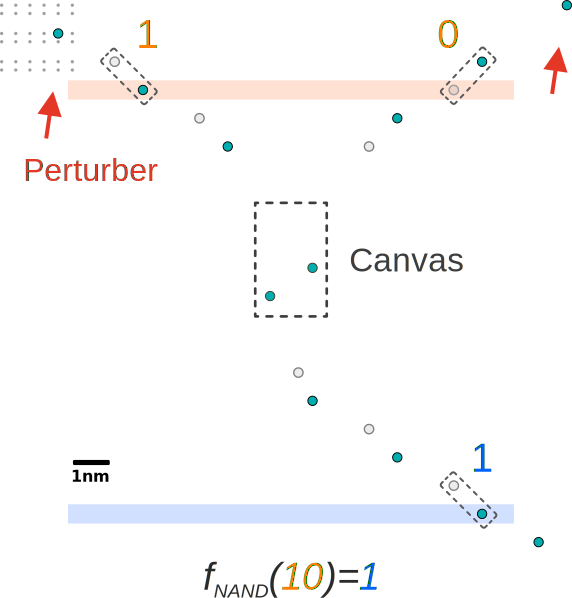
\includegraphics[width=.55\linewidth,valign=c]{figs/nand_10_bestagon_gate.pdf}
        \label{sfig:sidb-logic-hex-tile}
    }
    \caption{
        \TODO{Paraphrase.}
        \OLD{
        (\textbf{a}) A logic unit cell made of a pair of \glspl{sidb} sharing a single negative charge~\cite{huff2018binary} simulated in \emph{SiQAD}~\cite{ng2020siqad}. \textbf{Top:} the unit cell is illustrated without charges for readability; \textbf{middle:} unit cell simulated with charge, alongside an additional \gls{sidb} placed to the right (dubbed a \textit{perturber}), biasing the unit cell to take on logic state $0$; \textbf{bottom:} like above but with the perturber moved to the left, biasing the unit cell to take on logic $1$. Reprinted from~\cite{ng2023blueprint} with permission.
        (\textbf{b}) A \textsc{nand} gate from the \emph{Bestagon} library~\cite{walter2022hexagons} which defines standard locations for I/O pins and a canvas at the center which allows flexible placement of \glspl{sidb} to implement logic gates. Input pins are located at the top with input logic states set by input perturbers---a closer perturber pushes the input wire to the logic $1$ position, while a further one allows charges to take on logic $0$ state. The output is read out at the output pin located at the bottom. Adapted from~\cite{drewniok2025quicktrace} with permission.
        }
    }
    \label{fig:sidb-logic}
\end{figure}



\Glspl{sidb} can be manufactured on the surface of hydrogen-passivated Si(100)-2$\times$1 with the tip of a scanning-tunneling microscope \cite{achal2018lithography, huff2017atomic, pitters2024atomically}. Each \gls{sidb} is capable of holding discrete charge states, including negative, neutral, or positive. In densely packed ensembles, the charge state of each \gls{sidb} is determined by their collective interaction, bulk doping levels, and external electrostatic influences~\cite{pitters2024atomically}.
Binary logic states can be encoded by the position of a charge shared among closely positioned \glspl{sidb}, as illustrated in \fref{sfig:sidb-logic-pairs}, enabling the realization of logic gates such as an experimentally demonstrated \textsc{or} gate with a footprint of only $5\times\SI{6}{\nm^2}$~\cite{huff2018binary}.
Further exploration of \gls{sidb} gate and circuit designs~\cite{ahmadpour2023energyaware,vieira2022threeinput} was enabled by \emph{SiQAD}~\cite{ng2020siqad}, an open-source \gls{cad} tool and simulation environment for \gls{sidb} layouts. Building on these tools, the \emph{Bestagon} standard-tile library~\cite{walter2022hexagons} was introduced, featuring standardized \gls{io} pin locations and a central canvas on which \glspl{sidb} are placed to implement logic. A representative \textsc{nand} gate from this library is shown in \fref{sfig:sidb-logic-hex-tile}.
The \emph{Bestagon} library has allowed \emph{fiction}~\cite{walter2019fiction}, an \gls{eda} framework specialized for \gls{fcn} logic, to take gate-level netlists as input and synthesize dot-accurate, fabricable \gls{sidb} layouts~\cite{walter2022hexagons}, thus forming the backbone of this work.

\Gls{sidb} logic, like other \gls{fcn} families, uses spatially partitioned clock zones to enforce directed data flow~\cite{ng2020siqad, chiu2020poissolver}. Hanging or buried electrodes apply phase-shifted sinusoidal potentials that modulate the surface band bending and thereby the local charge density~\cite{chiu2020poissolver}. Adjacent electrodes are offset by \SI{90}{\degree} in phase, producing ``active'' regions where charges are present and computation occurs, separated by ``inactive'' regions that are effectively charge-free buffers. A simple, area-efficient arrangement places these clock zones in rows to support unidirectional, purely combinational logic~\cite{lent1997device,chiu2020poissolver}.
Interfacing with \gls{cmos} can be achieved by biasing inputs electrostatically via electrodes~\cite{chiu2020poissolver}, while outputs can be sensed using charge-sensitive devices such as single-electron transistors~\cite{fuechsle2012singleatom, prager2009integration, bohloul2017quantum}.

%%%%%%%%%%%%%%%%%%%%%%%%%%%%%%%%%%%%%%%%%%%%%%%%%%
% Related work
%%%%%%%%%%%%%%%%%%%%%%%%%%%%%%%%%%%%%%%%%%%%%%%%%%
\section{Related Work} \label{sec:related-work}

\begin{figure}
    \centering
    \includegraphics[width=0.95\linewidth]{figs/mxu.pdf}
    \caption{
        A 2D systolic array \gls{mxu} receiving quantized activations ($a$), weights ($w$), weight control signals ($C_w$), and partial sums ($s$). \Glspl{pe} inside the \gls{mxu} consist of a \gls{mac} unit, memory controller, and delay-line memory for weight storage. Signals propagate downward on the left side of the \gls{pe} (forward pass) and upwards on the right side (return pass).
        % \TODO{Consistent font size \& weight for I/O pins.} \TODO{Improve color scheme.} \TODO{Rounded corners in the right.}
    }
    \label{fig:mxu-systolic-array}
\end{figure}

Related \gls{fcn} design flows have been developed for \gls{nml}. \emph{ToPoliNano}~\cite{riente2017topolinano} provides a \gls{cmos}-like, top-down flow from structural VHDL descriptions to in-plane \gls{nml} layouts with clocking-aware placement, routing, and performance analysis.
Complementing this, \emph{FUNCODE}~\cite{garlando2021funcode} infers VHDL netlists from custom \gls{nml} layouts, enabling device-to-system analysis of \gls{nml} circuits using HDL simulators. These works demonstrate mature \gls{fcn} \gls{cad} capabilities in the \gls{nml} domain.
In contrast, the present work targets the emerging atomic-scale \gls{sidb} logic platform, for which a complete \gls{rtl}-to-atoms design flow for \gls{ml} accelerator workloads is demonstrated

Before dedicated \gls{sidb}-aware \gls{eda} tooling became available, studies of \gls{sidb} applications were limited and largely depended on manual \gls{cad} prototyping with extrapolated area and latency estimates.
One such example was an \gls{sidb} \gls{mxu}~\cite{ng2023blueprint} for \gls{ml} acceleration, which mirrored design choices from Google's \gls{tpu}v1~\cite{jouppi2017indatacenter}: the matrix-vector multiplications underpinning \gls{ml} workloads were realized as 8-bit integer \gls{mac} operations to reduce computational cost, and both designs employed a systolic-array architecture relying on regular arrangements of \glspl{pe}---homogeneous logic modules that operate on their inputs and pass results to adjacent \glspl{pe}---to perform computation (\fref{fig:mxu-systolic-array}).
At the \gls{pe} level, the core operation is a \gls{mac}: $s_{\text{out}} = s_{\text{in}} + (w \cdot a)$, where $s_\text{in}$ the incoming partial sum from the preceding \gls{pe}, $w$ is the stored weight, $a$ is the incoming activation, and $s_\text{out}$ is the updated partial sum.

In the implementation of~\cite{ng2023blueprint}, each matrix-multiplication job consisted of two primary phases:
%
\begin{enumerate*}
  \item \emph{preloading}, where weights ($w$) are loaded into the array from the top edge and transverse column-wise until each one arrives at the designated \gls{pe}, which stores them;
  \item \emph{computing}, where activations ($a$) are streamed from the left side and are multiplied with the stored weights and accumulated with partial sums; activations continue to transverse row-wise while partial sums transverse column-wise for further accumulation until they reach the array's bottom edge.
\end{enumerate*}
%
Additional input signals control the operating phase and the destination \gls{pe} index of each input weight.
At the \gls{pe} granularity, each \gls{pe} comprises two signal paths: a \emph{forward pass} containing the \gls{mac} and memory controller, and a \emph{return pass} that drives a weight bus upward to close the delay-line memory feedback loop and an activation bus to align activations with neighboring \glspl{pe}. As shown in \fref{fig:mxu-systolic-array}, both paths are purely combinational, enabling row-wise clocking on each path.
As row-wise clocking necessitates deep pipeline stages (\secref{sec:background}), at each clock cycle, different inputs can be interleaved to increase the computational throughput of the \gls{mxu}.


While that blueprint study reported promising area and power estimates against Google's \gls{tpu}v1~\cite{ng2023blueprint, jouppi2017indatacenter}, its extrapolated nature offered neither a manufacturable layout nor formal verification. The preceding conference version of this work~\cite{ng2025building} bridged this gap by demonstrating the first application\todo{Note to Marcel: to avoid overclaiming the conf paper's contribution, the wording claims that it \textit{applied} a synthesis flow rather than proposing it (since it didn't), please let me know whether this claim is clean enough; if there's still risk of being perceived as overclaiming I can further word smith this} of an \gls{rtl}-to-atoms synthesis flow to a quantized \gls{sidb} \gls{mxu}. This was achieved through a hierarchical \gls{rtl} structure that satisfied \gls{eda} tooling requirements while enabling clocking-level validation. This journal extension substantially refines that applied flow by introducing several technology-specific optimizations and exploring the scaling behavior of different quantization bit-widths, as detailed in the following section.





%%%%%%%%%%%%%%%%%%%%%%%%%%%%%%%%%%%%%%%%%%%%%%%%%%
% Methodology
%%%%%%%%%%%%%%%%%%%%%%%%%%%%%%%%%%%%%%%%%%%%%%%%%%
\section{Methodology} \label{sec:methodology}

This section details the end-to-end \gls{rtl}-to-atoms design and synthesis flow.
First, \secref{sec:methodology-verilog} describes the hierarchical \gls{rtl} Verilog architecture of the \gls{sidb} \gls{mxu}, which separates the combinational core from its clocked wrapper to satisfy \gls{eda} input constraints while enabling pipeline-level verification. Following this, the two-stage synthesis process is detailed: \secref{sec:methodology-rtl-to-netlist} covers the \gls{rtl}-to-netlist conversion, and \secref{sec:methodology-netlist-to-atoms} describes the netlist-to-atoms physical design, including several key optimizations introduced by this work.



\subsection{\titlecap{\glsentrylong{mxu} in Hierarchical RTL}}\label{sec:methodology-verilog}

\begin{algorithm}[tbp]
\footnotesize
\caption{Forward Pass Logic in Processing Element}\label{alg:pe-forward}

\renewcommand{\algorithmicrequire}{\textbf{Inputs:}}
\renewcommand{\algorithmicensure}{\textbf{Outputs:}}

\begin{algorithmic}[1]
    \newcommand{\codecomment}[1]{\textit{\textcolor{gray}{// #1}}}
    \Require
    \Statex $\mathit{PE}_{y} \gets$ y-index assigned to each PE (constant per PE)
    \Statex $m \gets$ PRELOAD (0) or COMPUTE (1) mode
    \Statex $w_\text{load} \gets$ weight to be loaded into memory
    \Statex $\mathit{PE}_{\text{target-}y} \gets$ target Y-index of $w_\text{load}$
    \Statex $s_\text{in} \gets$ input partial product
    \Statex $a \gets$ input activation
    \Statex $w_\text{mem} \gets$ weight loaded from delay-line memory

    \Ensure
    \Statex $s_\text{out}$: new partial sum
    \Statex $w_\text{memOut}$: weight to write to delay-line memory

    \Procedure{ProcessingElementLogic}{}
    \State $p \gets \text{signed}(w_\text{mem}) \times \text{signed}(a)$\Comment{Multiply stored $w$ with $a$}
    \State $p_\text{signExtended} \gets \text{signExtend}(p, 24)$
    \State $s_\text{out} \gets s_\text{in} + p_\text{signExtended}$\Comment{Sum with partial sum}
    \If{$m = \text{PRELOAD}$ \textbf{and} $PE_{\text{target-}y} = PE_{y}$}
       \State $w_\text{memOut} \gets w_\text{load}$\Comment{Update stored weight}
    \EndIf
    \State \Return $s_\text{out}$, $w_\text{memOut}$, and other pass-through wires
    \EndProcedure
\end{algorithmic}
\end{algorithm}

To achieve this work's objectives, the \gls{rtl} implementation must satisfy the following requirements:
%
\begin{enumerate*}
  \item the \gls{rtl} implementation must obey \emph{fiction}'s requirement for gate-level netlists to be purely combinational; and
  \item operation of the pipelined \gls{pe} must be verifiable so that test benches can establish operational correctness, addressing the lack of formal verification in prior work~\cite{ng2023blueprint}.
\end{enumerate*}
%
Because the \gls{pe} includes forward and return paths that form an internal feedback loop, a direct \gls{rtl} implementation of the full \gls{pe} would conflict with \emph{fiction}'s requirement for purely combinational gate-level netlists.
To reconcile these constraints, this work adopts a hierarchical \gls{rtl} organization, separating the design into a combinational core and a clocked shell:
%
\begin{description}
  \item[Combinational core:] The \gls{pe}'s forward-pass logic is implemented in strictly combinational \gls{rtl}, as shown in Alg.~\ref{alg:pe-forward}, ensuring compatibility with subsequent synthesis steps.
  \item[Clocked shell:] A higher-level \gls{rtl} module captures the clocked operation of the full \gls{pe}, defining the component's input and output signals, pipelined internal signal steering, and synchronized signal timing for the return pass.
\end{description}
%
Both the combinational core and the clocked shell are parameterized by the bit widths of weights and activations, allowing for a systematic study of how layout metrics scale with numerical precision in \secref{sec:results}.

Correctness was validated with test benches across the stack, including both the combinational core and the clocked shell. These tests confirmed correct weight storage in preload mode and accurate \gls{mac} results in compute mode for representative input activations, stored weights, and partial sums.
In particular, interleaved inputs for concurrent \gls{mac} operation across all pipeline stages was also verified. All simulations were performed using Icarus Verilog~\cite{icarusverilog}. The logical correctness of the \gls{pe} was thus established prior to synthesis and physical mapping. The full open-source codebase is available on GitHub~\cite{githubsupplementary}\todo{Check code prior to final submission}.

\subsection{RTL-to-Netlist}\label{sec:methodology-rtl-to-netlist}


With the \gls{rtl} design verified, the first stage of the synthesis flow is to generate a gate-level netlist. To accomplish this, this work uses \emph{Yosys}~\cite{wolf2013yosys} to map arithmetic operators such as \mbox{accumulation (\texttt{+})} and \mbox{multiplication (\texttt{*})} into gate-level \glspl{alu}.
Absent explicit directives, \emph{Yosys} selects \gls{cmos}-optimized \gls{alu} implementations, which can underperform in \gls{fcn} because their strictly planar fabrics force gates and wires to share the same plane, altering the area and latency trade-offs \cite{kim2010multipliers}. To ensure technology-appropriate choices, this work supplies explicit gate-level descriptions of a ripple-carry adder and an array multiplier to the \emph{Yosys} technology mapper. These implementations have been shown to suit \gls{fcn} technologies thanks to their regular structure, which eases wiring congestion and limits the need for crossovers \cite{kim2010multipliers}.
The mapped netlist is then rewritten as an \gls{aig} with \emph{Yosys} and optimized with ABC's \textit{\&deepsyn}~\cite{brayton2010abc} strategy to reduce the network's node count.
Finally, the resulting gate-level netlist is validated against the \gls{pe}-core test benches to confirm functional correctness.

\subsection{Netlist-to-Atoms}\label{sec:methodology-netlist-to-atoms}

The gate-level netlist is then passed to the \emph{fiction} framework~\cite{walter2019fiction} for the second stage of the synthesis flow: physical design. This stage transforms the netlist into a dot-accurate \gls{sidb} layout through a multi-step process, which this work enhances with several optimizations for the \gls{sidb} platform.

\subsubsection{\textit{fiction} Synthesis Flow}

The verified gate-level netlist is subsequently forwarded to \emph{fiction}~\cite{walter2019fiction}, whose \gls{fcn}-aware toolchain synthesizes it into an \gls{sidb} layout following the synthesis flow proposed by \cite{walter2022hexagons}:
%
\begin{enumerate}
  \item Technology mapping maps the \gls{aig} onto the \emph{Bestagon} gate library~\cite{walter2022hexagons}, exploiting the library's richer primitives to shrink the logic compared with an AND/INV-only basis.
  \item Placement and routing with the \textit{ortho}~\cite{walter2019scalable} or \gls{gold}~\cite{hofmann2024born} algorithm produces a layout on a Cartesian grid.
  \item \Gls{plo}~\cite{hofmann2023postlayout, hofmann2024late} reduces the footprint of the routed design.
  \item The Cartesian layout is projected onto a hexagonal grid~\cite{hofmann2023scalable} in preparation for applying the \emph{Bestagon} gates.
  \item SAT-based equivalence checking~\cite{walter2020verification} confirms that the hexagonalized layout preserves the gate-level behavior.
  \item The \emph{Bestagon} library~\cite{walter2022hexagons} is applied to the verified layout, yielding a dot-accurate, manufacturable \gls{sidb} layout.
\end{enumerate}
%
While this established workflow provides a robust foundation, its application to the \gls{sidb} platform revealed opportunities for technology-specific enhancements, which are detailed below and further examined in \secref{sec:results}.

\subsubsection{FoM-aware Technology Mapping}

Previous \gls{sidb} synthesis flows within \emph{fiction} treated all gates in the technology library as equivalent, without considering their physical robustness.
Recent advancements in \gls{sidb} logic robustness studies have culminated in the creation of a unified cost function for \glspl{fom} for \gls{sidb} gates~\cite{drewniok2024unifying}. The cost function encompasses the dominant cost drivers---operational domain size~\cite{ng2020siqad, walter2023reducing}, thermal stability~\cite{drewniok2023temperature}, band-bending effects~\cite{pitters2011charge}, defect sensitivity~\cite{ng2024simulating, huff2019electrostatic, croshaw2020atomic}, and related factors---into a single score $\chi$.
This work adopts $\chi$ as the objective for the technology mapper so that the flow prioritizes gates with higher predicted robustness, accepting a potential trade-off in other layout metrics like area or device count.

\subsubsection{Placement and Routing Improvements for SiDBs}\label{subsubsec:methodology-p-and-r-improvements-for-sidb}

The placement-and-routing framework within \emph{fiction} was first established for \gls{qca} circuits on a Cartesian grid under a 2DDWave clocking scheme~\cite{walter2019fiction}. Subsequent support for \gls{sidb} logic was enabled through a coordinate mapping that involves a $45^\circ$ rotation of the Cartesian layout prior to its projection onto the hexagonal \gls{sidb} lattice~\cite{hofmann2023scalable}.
This rotation, however, can lead to suboptimal results; a layout that is compact on the Cartesian grid may become significantly larger after hexagonalization because horizontal and vertical paths are transformed into longer diagonal routes.
While the older \emph{ortho} algorithm offers no configuration to compensate for this, the more recent \gls{gold} algorithm~\cite{hofmann2024born} exposes a configurable cost objective for placement and routing, enabling optimizations more suitable for the final \gls{sidb} layout.
Whereas the default cost objective for \gls{gold} is the area, this work introduces new cost objectives that encourage more square footprints and to reduce the aspect-ratio distortion introduced by the $45^\circ$ rotation during the hexagonalization step; they are detailed in \secref{sec:results-synthesis-metrics}.

\subsubsection{Hexagonalization Improvements}

The hexagonalization algorithm was also revised in this work to align generated layouts with \gls{sidb} clocking expectations. Under the Cartesian layout's 2DDWave clocking scheme~\cite{vankamamidi2008twodimensional}, primary inputs are placed along the north and west borders and data advances diagonally toward the southeast. The $45^\circ$ rotation applied during hexagonalization left many inputs and outputs recessed from the north and south edges, respectively. These offsets reduce the attainable throughput because some signals must be held across multiple cycles for synchronization. The updated flow stretches all input and output pins to the north and south boundaries after projection, producing layouts whose ports are time-aligned as they enter and exit the hexagonal fabric.

%%%%%%%%%%%%%%%%%%%%%%%%%%%%%%%%%%%%%%%%%%%%%%%%%%
% Experimental Results
%%%%%%%%%%%%%%%%%%%%%%%%%%%%%%%%%%%%%%%%%%%%%%%%%%
\section{Experimental Results}\label{sec:results}

This section evaluates the \gls{rtl}-to-atoms flow using the synthesized \gls{pe}-core layouts.
First, \secref{sec:results-experimental-protocol} outlines the experimental protocol, including the considered quantization settings and physical-design configurations.
Then, \secref{sec:results-synthesis-metrics} presents the resulting synthesis metrics across technology-mapping and placement-and-routing variants.
Finally, \secref{sec:results-discussion} discusses these findings in the context of prior manual estimations and the remaining opportunities for optimization.

\begin{table*}
  \caption{Extended synthesis comparison across quantization and routing settings}
  \centering
  \label{tab:pe-results-extended}
  \begin{minipage}{\linewidth}
    \centering
    \begin{tabular}{l@{\hskip 6pt}l@{\hskip 6pt}l@{\hskip 12pt}
                    r@{~$\times$~}l@{~$=$~}r@{\hskip 12pt}
                    r@{~$\times$~}l@{~$=$~}r@{\hskip 4pt}
                    @{(}r@{\hskip 0.25em}S[table-format=3.2]@{\hskip 0.25em \%)}}
      \toprule
      \multirow[c]{2}{*}{\makecell[tl]{\textsc{Experiment}}} &
      \multirow[c]{2}{*}{\makecell[tl]{\textsc{PE}}} &
      \multirow[c]{2}{*}{\makecell[tl]{\textsc{Alg}}} &
      \multicolumn{3}{c}{\textsc{Uniform TM}} &
      \multicolumn{5}{c}{\textsc{FoM-aware TM}} \\
      \cmidrule(lr{12pt}){4-6} \cmidrule(lr){7-11}
        & & & $w$ & $h$ & $A_\text{uni}$ & $w$ & $h$ & $A_\text{FoM}$ & \multicolumn{2}{r}{\textsc{vs} $A_\text{uni}$)} \\
      \midrule
      Default \glspl{alu}~\cite{ng2025building} & W8A8 & \emph{ortho} &
      \num{515} & \num{1043} & \num{537145} &
      \num{516} & \num{1049} & \num{541284} & + & 0.77 \\
      \cmidrule(lr){1-11}
      \multirow[t]{5}{*}{\makecell[tl]{Optimized \glspl{alu}\\(This work)}} & W8A8 & \emph{ortho} &
      \num{474} & \num{967} & \num{458358} &
      \num{478} & \num{985} & \num{470830} & + & 2.72 \\[0.8ex]
        & \multirow[t]{2}{*}{W4A4} & \emph{ortho} &
      \num{143} & \num{333} & \num{47619} &
      \num{164} & \num{346} & \num{56744} & + & 19.16 \\
        &  & \emph{gold} &
      \num{116} & \num{241} & \num{27956} &
      \num{182} & \num{385} & \num{70070} & + & 150.64 \\[0.8ex]
        & \multirow[t]{2}{*}{W2A2} & \emph{ortho} &
      \num{67} & \num{151} & \num{10117} &
      \num{69} & \num{157} & \num{10833} & + & 7.08 \\
        &  & \emph{gold} &
      \num{48} & \num{98} & \num{4704} &
      \num{51} & \num{107} & \num{5457} & + & 16.01 \\
      \bottomrule
    \end{tabular}
    \begin{minipage}{\linewidth}
      \footnotesize
      \vspace{0.5em}
      Here $w$, $h$, and $A$ denote the tile counts along width, height, and footprint ($A = w \times h$); ``uniform TM'' and ``\gls{fom}-aware TM'' denote the Bestagon variant used for technology mapping; ``vs $A_\text{uni}$'' reports the percentage change imposed by \gls{fom}-aware technology mapping. ``Default'' and ``optimized'' \glspl{alu} indicate whether adder/multiplier selection was left to \emph{Yosys}'s defaults or specifically defined. %\TODO{Do a final check with sweep data to make sure the reported minimums accurately reflect latest results.}
    \end{minipage}
  \end{minipage}
\end{table*}

\begin{table}
  \caption{Cost objective comparison for \emph{gold} algorithm}
  \centering
  \label{tab:gold-cost-comparison}
  \begin{minipage}{\linewidth}
    \centering
      \begin{tabular}{l@{\hskip 4pt}l@{\hskip 8pt}
                      r@{\hskip 3pt}r@{\hskip 8pt}
                      r@{\hskip 3pt}r}
        \toprule
        \textsc{PE} &
        \textsc{Cost obj} &
        \multicolumn{2}{l}{$A_\mathrm{min}$} &
        \multicolumn{2}{l}{$\bar{A}$} \\
        \midrule
        \multirow[t]{3}{*}{\makecell[tl]{W4A4}} & Area (baseline) &
        \num{27956} &  &
        \num{37483.61} & \\
         & $x + y$ &
        \num{27956} & $(+\SI{0.00}{\percent})$ &
        \num{37303.28} & $(\SI{-0.48}{\percent})$ \\
         & $x^{2} + y^{2}$ &
        \num{28175} & $(+\SI{0.78}{\percent})$ &
        \num{36716.71} & $(\SI{-2.05}{\percent})$ \\
        \cmidrule(lr){1-6}
        \multirow[t]{3}{*}{\makecell[tl]{W2A2}} & Area (baseline) &
        \num{5145} & &
        \num{10156.22} & \\
         & $x + y$ &
        \num{5145} & $(+\SI{0.00}{\percent})$ &
        \num{8107.02} & $(\SI{-20.18}{\percent})$ \\
         & $x^{2} + y^{2}$ &
        \num{4704} & $(\SI{-8.57}{\percent})$ &
        \num{8121.47} & $(\SI{-20.03}{\percent})$ \\
        \bottomrule
      \end{tabular}
      \begin{minipage}{\linewidth}
        \footnotesize
        \vspace{0.5em}
        $A_\mathrm{min}$ and $\bar{A}$ represent the minimum and mean areas for that combination of array and \gls{gold} cost objective.
        Uniform technology mapping was used.
        The percentage differences report synthesized areas compared against the ``area'' cost objective.
        All trials ran \gls{gold} in single-core mode with a timeout of \SI{400}{\second} on an AMD Ryzen 9 9950X3D with maximum effort mode, primary input tile skipping was swept from \numrange{1}{6} with randomization enabled. $630$ trials were performed per configuration, with unsuccessful results discarded.
        \gls{plo} was performed for all trials with maximum gate relocations restricted to $1$.
      \end{minipage}
  \end{minipage}
\end{table}

\subsection{Experimental Protocol}\label{sec:results-experimental-protocol}

This comparative study aims to showcase the scaling behavior of various bit-width configurations for activations and weights, as well as the synthesis results under various configurations for the technology mapper and placement-and-routing algorithms.
To this end, the combinational \gls{pe}-core (\secref{sec:methodology-verilog}) is synthesized for 2-, 4-, and 8-bit weights and activations, henceforth denoted W2A2, W4A4, and W8A8, respectively.
These selections correspond to widely studied quantized regimes for CNNs and Transformers where the dominant operations reduce to matrix multiplications that map directly onto an \gls{mxu} \cite{esser2020learnedstepsizequantization, banner2019post, jouppi2017indatacenter}.

The \gls{rtl}-to-netlist flow from this work instructs \emph{Yosys} to use ripple-carry adders for accumulation and array multipliers for multiplication to produce an \gls{aig}, which is then optimized using ABC's \emph{\&deepsyn} strategy~\cite{brayton2010abc}. %On a AMD Ryzen 9 3900X CPU, \emph{\&deepsyn} reached its internal iteration limit at \SI{0.4}{\hour}, \SI{1}{\hour}, and \TODO{} for W2A2, W4A4, and W8A8, respectively.
As for the netlist-to-atoms flow, the \emph{Bestagaon} library~\cite{walter2022hexagons} is used. Technology mapping with uniform cost serves as the baseline for comparison with \gls{fom}-aware counterparts. For placement and routing, results from \emph{ortho} and \gls{gold} are reported if valid layouts were achieved; \gls{plo} is always performed.

\subsection{Results}\label{sec:results-synthesis-metrics}

The best achieved synthesis results of the \gls{pe}-core under various configurations are presented in \tref{tab:pe-results-extended}.
Compared to the prior results, which allowed \emph{Yosys} to select its default CMOS-aligned \glspl{alu}~\cite{ng2025building}, explicitly constraining \emph{Yosys} to initiate \glspl{alu} optimized for \gls{sidb} logic yields a \SI{15}{\percent} area reduction, underscoring the importance of specifying technology-appropriate logic components.
Turning to the \gls{fom}-informed technology mapping results, the corresponding layouts are consistently larger than those obtained by treating all gates with equal preference, indicating that the technology mapper has chosen costlier solutions that make use of more robust gates as expected. This trade-off in area comes with the benefit that \gls{sidb} gates with higher reliability metrics are more often employed in the layout, which can ultimately yield a more robust device. It is also important to note that the \gls{fom} values from~\cite{drewniok2024unifying} are derived from a specific variant of the \emph{Bestagon} library optimized for a particular set of physical conditions. Choosing or designing different libraries tailored to specific physical conditions may yield different trade-offs.

On the choice of placement and routing algorithms, while the W8A8 configuration has a gate-level netlist that exceeds \gls{gold}'s practical problem range, W4A4 and W2A2 remain sufficiently small for \gls{gold} to successfully place and route layouts, achieving a $\approx\!40\text{--}50\,\%$ area reduction relative to their \emph{ortho}-based counterparts. In the \gls{fom}-aware results, however, a pronounced area increase arises for W4A4, where the layout produced by \gls{gold} is even larger than that from \emph{ortho}. This work interprets that outlier as evidence that, under \gls{fom}-aware technology mapping, the resulting netlist is already near the upper bounds of \gls{gold}'s ability to provide consistent solutions: among $630$ trials for this configuration, only $1$ produced a completed placed and routed layout. Nevertheless, for configurations that remain within \gls{gold}'s effective scaling regime, it delivers area reductions that directly translate to improved manufacturability and reduced power consumption in practice.

Part of the improvement achieved with \gls{gold} arises from refining the cost objectives in the \gls{sidb}-specific synthesis workflow (\secref{subsubsec:methodology-p-and-r-improvements-for-sidb}). Two additional \gls{gold} cost objectives were implemented---Manhattan distance ($x+y$) and squared Euclidean distance ($x^2+y^2$)---and compared against the default area-based objective in \tref{tab:gold-cost-comparison}. For the W2A2 configuration, both the best and average layout areas improve, with the gains being more pronounced in the average case and the squared Euclidean objective yielding the smallest minimum area. For W4A4, modest improvements persist in the average case, but no benefit is observed in the minimum area. This behavior is consistent with W4A4 already operating near the upper end of \gls{gold}'s practical scaling range, where a reduced number of successful runs can skew the distribution of best-case results.

\subsection{Discussion}\label{sec:results-discussion}

The synthesized \gls{sidb} layouts implement the \gls{pe}-core, which represents all the logic operations in the \gls{pe}; the omitted parts are purely for signal propagation~(\secref{sec:methodology-verilog}).
A full \gls{pe}-level estimation would additionally require routing the \gls{io} pins of the \gls{pe}-core to the outer \gls{io} of the \gls{pe} module and accounting for the wiring cost of the return pass. Automating these steps calls for further streamlining of \gls{sidb} \gls{eda} tools and is therefore left as future work.

Despite this estimation gap, the \gls{pe}-core captures the computational portion of the \gls{pe}, making it meaningful to compare the synthesis results against the manual \gls{sidb} \gls{mxu} estimates from~\cite{ng2023blueprint}.
Using the tile dimensions in \tref{tab:pe-results-extended}, the physical dimensions can be computed by $w \times \SI{23.06}{\nano\meter}$ and $h \times \SI{13.06}{\nano\meter}$.\footnote{These scaling factors differ from~\cite{ng2025building} due to corrected calculation factors employed in this work.}
Relative to the manually estimated dimensions of $5000 \times \SI{8150}{\nano\meter^2}$~\cite{ng2023blueprint}, the synthesized layout using optimized \glspl{alu} represent a $3.4\times$ increase in area use; the gap would further widen if the entire \gls{pe} was synthesized.

Several factors contribute to this discrepancy. Whereas the manual estimation used hand-designed components with relatively high logic gate density~\cite{ng2023blueprint}, this work employs the \emph{Bestagon} gate library, whose larger tile template deliberately ensures sufficient separation between the logic canvases of neighboring tiles to minimize inter-gate interference~\cite{walter2022hexagons}. In addition, while the manual estimation directly employed optimized \gls{alu} layouts, this work can only influence \gls{alu} selection at the \gls{rtl}-to-netlist synthesis stage via \emph{Yosys}; after ABC's netlist optimization, the boundaries of arithmetic elements become blurred, limiting the effectiveness of optimization algorithms that could exploit arithmetic structure. Finally, the large W8A8 netlist is computationally intractable for \gls{gold} to place and route, preventing the $\approx40\text{--}50\,\%$ area reductions observed for smaller configurations from being realized at this bit-width. Nevertheless, the successful end-to-end design flow achieved in this work demonstrates what state-of-the-art \gls{fcn} \gls{eda} tools can realize on the \gls{sidb} platform, combining manufacturable layouts with full testbench-based verification and highlighting opportunities for further optimization.

%%%%%%%%%%%%%%%%%%%%%%%%%%%%%%%%%%%%%%%%%%%%%%%%%%
% Future Work
%%%%%%%%%%%%%%%%%%%%%%%%%%%%%%%%%%%%%%%%%%%%%%%%%%
\section{Conclusion and Future Work}\label{sec:conclusion-future-work}

\OLD{In past studies, the design and verification of large-scale SiDB applications remained disconnected from their physical implementations, constrained by immature \gls{eda} tooling and manually-intensive workflows at the time~\cite{chiu2020thes, ng2023blueprint}. Enabled by recent advances in \gls{sidb}-focused \gls{eda} frameworks, this work presents the first automated, end-to-end design flow for implementing a processing element (\gls{pe}) of a \gls{sidb}-based \glsentrylong{mxu} designed specifically for \gls{ml} acceleration.
Our hierarchical Verilog structure facilitates the synthesis of combinational components down to the \gls{sidb} level while enabling validation of the complete operational functionality through higher-level \gls{rtl} modules. By strategically separating core combinational logic from higher-level pipeline control, we successfully synthesized a majority of the \gls{pe}'s functionality into a dot-accurate \gls{sidb} layout, selectively omitting specific signal components from synthesis to accommodate \gls{eda} tooling restrictions. Although the synthesized layout exhibits a larger area compared to previous hand-crafted designs~\cite{ng2023blueprint}, our effort provides a concrete demonstration of automated design methodologies applied to \gls{sidb}-based circuits, and underscores opportunities for further optimizations in \gls{sidb}-specific \gls{eda} flows. Additionally, this study is the first to incorporate \gls{fom} considerations into \emph{fiction}'s technology mapping process, prioritizing gate reliability within synthesized layouts.}

\OLD{One limitation faced by this study is the lack of control over the implementation of fundamental arithmetic units such as adders and multipliers. Since the design trade-offs of \gls{sidb} logic differ significantly from CMOS designs, it is possible that our workflow for synthesizing \gls{rtl} Verilog to gate-level Verilog using established tools like Yosys and ABC is introducing unnecessary overhead due suboptimal implementation choices. Further improvements to this synthesis step, as well as further developments to \emph{fiction}'s placement and routing algorithms, can bridge the gap between synthesized layouts and expert-designs and incentivize further development of novel applications optimized for \glspl{sidb}.}


%%%%%%%%%%%%%%%%%%%%%%%%%%%%%%%%%%%%%%%%%%%%%%%%%%
% Bibliography
%%%%%%%%%%%%%%%%%%%%%%%%%%%%%%%%%%%%%%%%%%%%%%%%%%
\bibliographystyle{IEEEtran}
\bibliography{zotero_refs_2025,manual_refs}
% zotero_refs.bib: original bib file exported from Zotero
% zotero_refs_normalized.bib: modified bib file where author fields with >6 authors are converted to et al



\end{document}
